
\documentclass{article}[14pt]
\usepackage{multicol, enumerate, enumitem, hyperref, color, soul, setspace, parskip, fancyhdr, amssymb, amsthm, amsmath, bbm, latexsym, units, mathtools}
\everymath{\displaystyle}
\usepackage[headsep=0.5cm,headheight=0cm, left=1 in,right= 1 in,top= 1 in,bottom= 1 in]{geometry}
\pagestyle{fancy}
\lhead{}
\chead{Answer Key for Module\,6\,-\,Polynomial\,Functions Version A}
\rhead{}
\lfoot{Summer\,C\,2020}
\cfoot{}
\rfoot{}
\begin{document}
\textbf{This key should allow you to understand why you choose the option you did (beyond just getting a question right or wrong). \href{https://xronos.clas.ufl.edu/mac1105spring2020/courseDescriptionAndMisc/Exams/LearningFromResults}{More instructions on how to use this key can be found here}.}

\textbf{If you have a suggestion to make the keys better, \href{https://forms.gle/CZkbZmPbC9XALEE88}{please fill out the short survey here}.}

\textit{Note: This key is auto-generated and may contain issues and/or errors. The keys are reviewed after each exam to ensure grading is done accurately. If there are issues (like duplicate options), they are noted in the offline gradebook. The keys are a work-in-progress to give students as many resources to improve as possible.}

\rule{\textwidth}{0.4pt}

26. Construct the lowest-degree polynomial given the zeros below. Then, choose the intervals that contain the coefficients of the polynomial in the form $x^3+bx^2+cx+d$.
$$ -5 + 4i \text{ and } -4 $$ 
The solution is $ x^{3} +14 x^{2} +81 x + 164 $ 

\begin{enumerate}[label=\Alph*.] 
\item $ b \in [13, 20], c \in [77, 87], \text{ and } d \in [161, 165] $ 

 * $x^{3} +14 x^{2} +81 x + 164$, which is the correct option. 
\item $ b \in [-22, -9], c \in [77, 87], \text{ and } d \in [-169, -163] $ 

 $x^{3} -14 x^{2} +81 x -164$, which corresponds to multiplying out $(x-(-5 + 4i))(x-(-5 - 4i))(x -4)$. 
\item $ b \in [-5, 7], c \in [-2, 4], \text{ and } d \in [-17, -8] $ 

 $x^{3} + x^{2} -16$, which corresponds to multiplying out $(x -4)(x + 4)$. 
\item $ b \in [-5, 7], c \in [7, 11], \text{ and } d \in [19, 22] $ 

 $x^{3} + x^{2} +9 x + 20$, which corresponds to multiplying out $(x + 5)(x + 4)$. 
\item $ \text{None of the above.} $ 

 This corresponds to making an unanticipated error or not understanding how to use nonreal complex numbers to create the lowest-degree polynomial. If you chose this and are not sure what you did wrong, please contact the coordinator for help. 
\end{enumerate} 
 
General Comments: Remember that the conjugate of $a+bi$ is $a-bi$. Since these zeros always come in pairs, we need to multiply out $(x-(-5 + 4i))(x-(-5 - 4i))(x-(-4))$.

-----------------------------------------------

27. Describe the end behavior of the polynomial below.
$$ f(x) = 9(x - 6)^{3}(x + 6)^{4}(x + 5)^{2}(x - 5)^{4} $$ 

 
 The solution is  
 \begin{center} 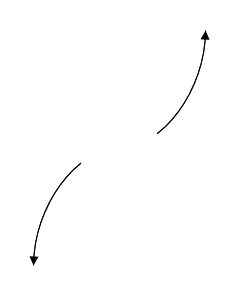
\includegraphics[width=0.3\textwidth]{../Figures/endBehaviorPositiveOddA.png} \end{center}\begin{tabular}{|c|c|} 
\hline 
 & \tabularnewline 
 \textbf{A.} 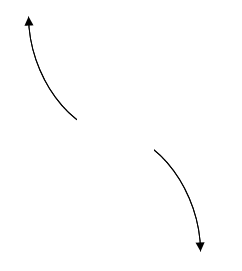
\includegraphics[width=0.3\textwidth]{../Figures/endBehaviorNegativeOddA.png} & \textbf{B.} 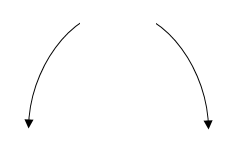
\includegraphics[width=0.3\textwidth]{../Figures/endBehaviorNegativeEvenA.png} \tabularnewline 
\hline 
 & \tabularnewline 
 \textbf{C.} 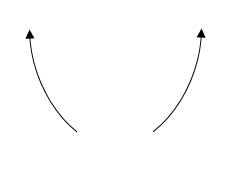
\includegraphics[width=0.3\textwidth]{../Figures/endBehaviorPositiveEvenA.png} & \textbf{D.} 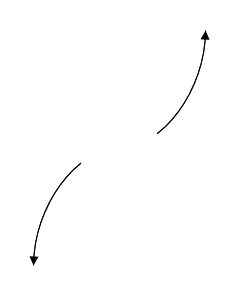
\includegraphics[width=0.3\textwidth]{../Figures/endBehaviorPositiveOddA.png} \tabularnewline 
\hline 
 E. None of the figures above. & \tabularnewline 
\hline 
 \end{tabular} 
 
\textbf{General Comments:} Remember that end behavior is determined by the leading coefficient AND whether the \textbf{sum} of the multiplicities is positive or negative.

-----------------------------------------------

28. Construct the lowest-degree polynomial given the zeros below. Then, choose the intervals that contain the coefficients of the polynomial in the form $ax^3+bx^2+cx+d$.
$$ \frac{-1}{2}, 6, \text{ and } \frac{-1}{4} $$ 
The solution is $ 8x^{3} -42 x^{2} -35 x -6 $ 

\begin{enumerate}[label=\Alph*.] 
\item $ a \in [0, 16], b \in [43, 49], c \in [-17, -4], \text{ and } d \in [-15, -3] $ 

 $8x^{3} +46 x^{2} -13 x -6$, which corresponds to multiplying out $(2x + 2)(x + 1)(4x -4)$. 
\item $ a \in [0, 16], b \in [-49, -38], c \in [-41, -25], \text{ and } d \in [-15, -3] $ 

 * $8x^{3} -42 x^{2} -35 x -6$, which is the correct option. 
\item $ a \in [0, 16], b \in [-49, -38], c \in [-41, -25], \text{ and } d \in [1, 9] $ 

 $8x^{3} -42 x^{2} -35 x + 6$, which corresponds to multiplying everything correctly except the constant term. 
\item $ a \in [0, 16], b \in [41, 44], c \in [-41, -25], \text{ and } d \in [1, 9] $ 

 $8x^{3} +42 x^{2} -35 x + 6$, which corresponds to multiplying out $(2x -1)(x + 6)(4x -1)$. 
\item $ a \in [0, 16], b \in [-57, -48], c \in [10, 13], \text{ and } d \in [1, 9] $ 

 $8x^{3} -50 x^{2} +11 x + 6$, which corresponds to multiplying out $(2x + 2)(x -1)(4x -4)$. 
\end{enumerate} 
 
General Comments: To construct the lowest-degree polynomial, you want to multiply out $(2x + 1)(x -6)(4x + 1)$

-----------------------------------------------

29. Which of the following equations \textit{could} be of the graph presented below?
\begin{center} 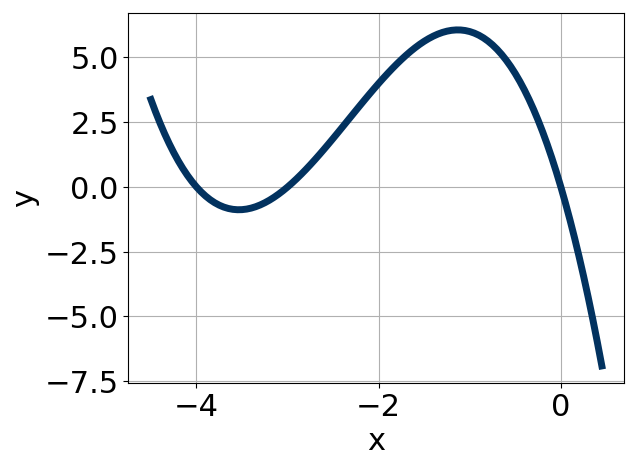
\includegraphics[width=0.3\textwidth]{../Figures/polyGraphToFunctionA.png} \end{center} 

The solution is $ 7x^{9} (x - 2)^{8} (x - 1)^{9} $ 

\begin{enumerate}[label=\Alph*.] 
\item $ -14x^{7} (x - 2)^{6} (x - 1)^{5} $ 

 This corresponds to the leading coefficient being the opposite value than it should be. 
\item $ -3x^{8} (x - 2)^{4} (x - 1)^{7} $ 

 The factor $x$ should have an odd power and the leading coefficient should be the opposite sign. 
\item $ 7x^{9} (x - 2)^{8} (x - 1)^{9} $ 

 * This is the correct option. 
\item $ 19x^{9} (x - 2)^{7} (x - 1)^{4} $ 

 The factor $2$ should have an even power and the factor $1$ should have an odd power. 
\item $ 9x^{7} (x - 2)^{10} (x - 1)^{8} $ 

 The factor $(x - 1)$ should have an odd power. 
\end{enumerate} 
 
General Comments: Draw the x-axis to determine which zeros are touching (and so have even multiplicity) or cross (and have odd multiplicity).

-----------------------------------------------

30. Describe the zero behavior of the zero $x = -6$ of the polynomial below.
$$ f(x) = 6(x + 6)^{3}(x - 6)^{4}(x + 3)^{4}(x - 3)^{7} $$ 

 
 The solution is  
 \begin{center} 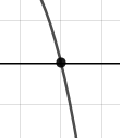
\includegraphics[width=0.3\textwidth]{../Figures/zeroBehaviorNegativeOddA.png} \end{center}\begin{tabular}{|c|c|} 
\hline 
 & \tabularnewline 
 \textbf{A.} 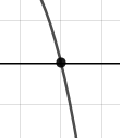
\includegraphics[width=0.3\textwidth]{../Figures/zeroBehaviorNegativeOddA.png} & \textbf{B.} 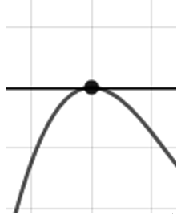
\includegraphics[width=0.3\textwidth]{../Figures/zeroBehaviorNegativeEvenA.png} \tabularnewline 
\hline 
 & \tabularnewline 
 \textbf{C.} 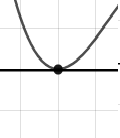
\includegraphics[width=0.3\textwidth]{../Figures/zeroBehaviorPositiveEvenA.png} & \textbf{D.} 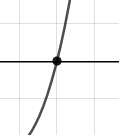
\includegraphics[width=0.3\textwidth]{../Figures/zeroBehaviorPositiveOddA.png} \tabularnewline 
\hline 
 E. None of the figures above. & \tabularnewline 
\hline 
 \end{tabular} 
 
\textbf{General Comments:} You will need to sketch the entire graph, then zoom in on the zero the question asks about.

-----------------------------------------------


\end{document}

